\documentclass[tikz, border=50pt]{standalone}

\usepackage{tikz}
\usepackage{medl_colors}
\usepackage{graphicx}
\usetikzlibrary{shapes.multipart, shapes.geometric, arrows.meta}
\usetikzlibrary{matrix, calc, positioning,fit}
\usepackage{xstring}

\begin{document}
\begin{tikzpicture}

%input picture
\node[scale = .5] (aepoints)  {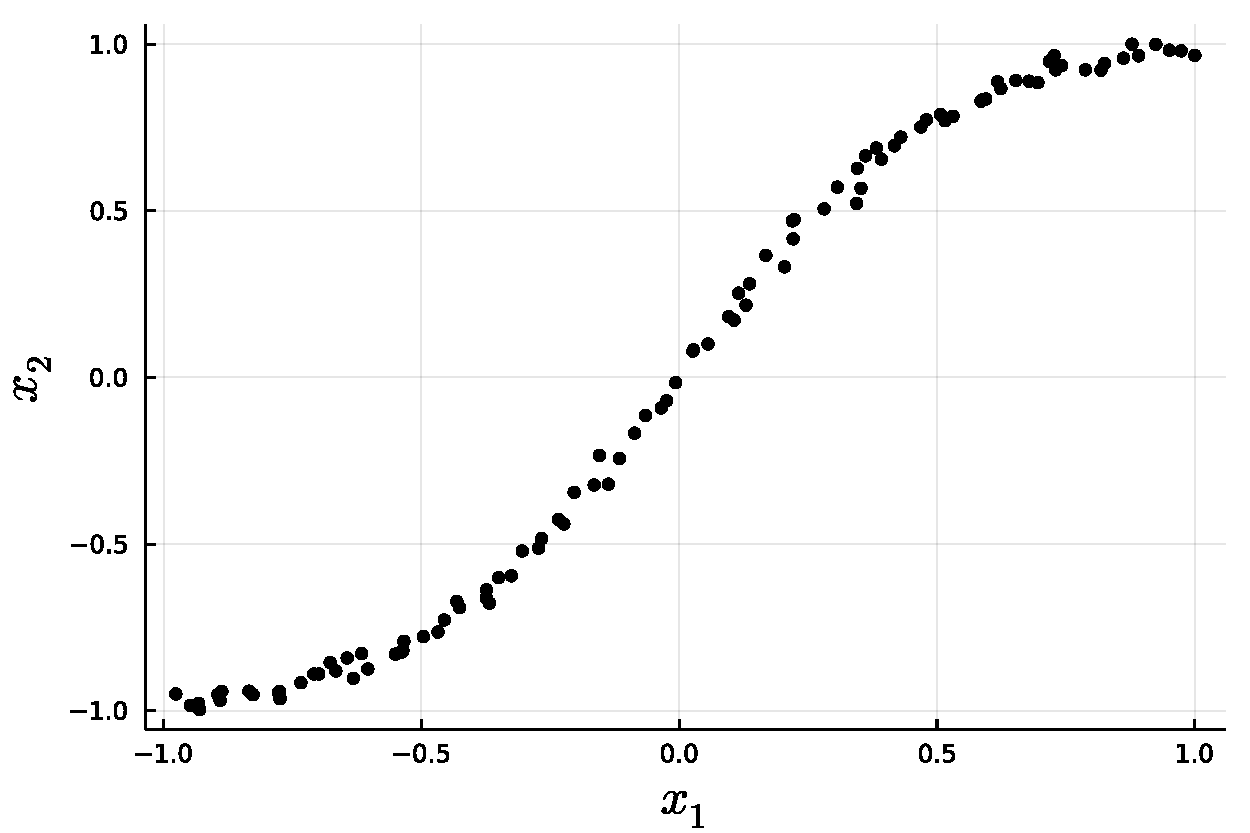
\includegraphics {images/ae_points.pdf}};

\node[scale = .2, below of=aepoints, node distance=30cm, xshift=-14cm] (pcacodepoints)  {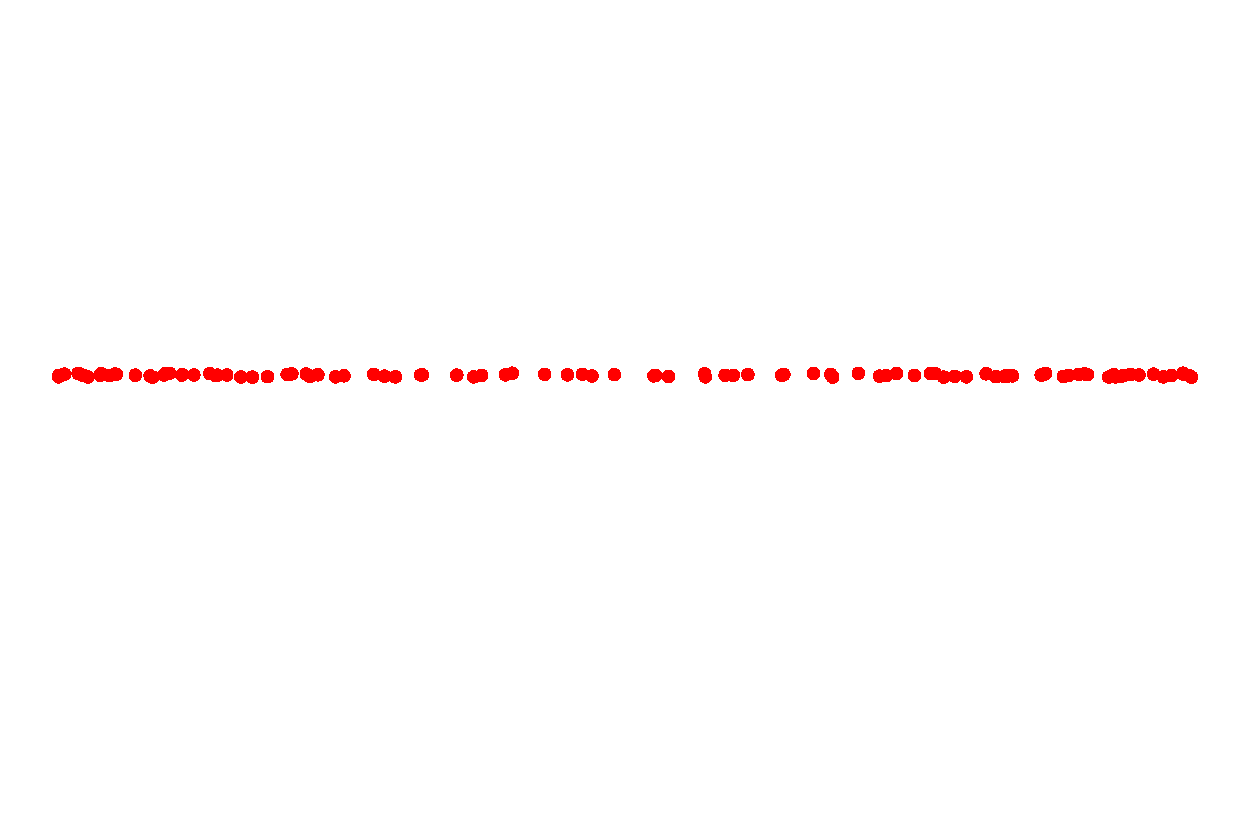
\includegraphics[trim={0 6cm 0 5cm},clip] {images/pca_code_points.pdf}};
\node[scale = .2, below of=aepoints, node distance=30cm, xshift=14cm,  rotate=180] (aecodepoints)  {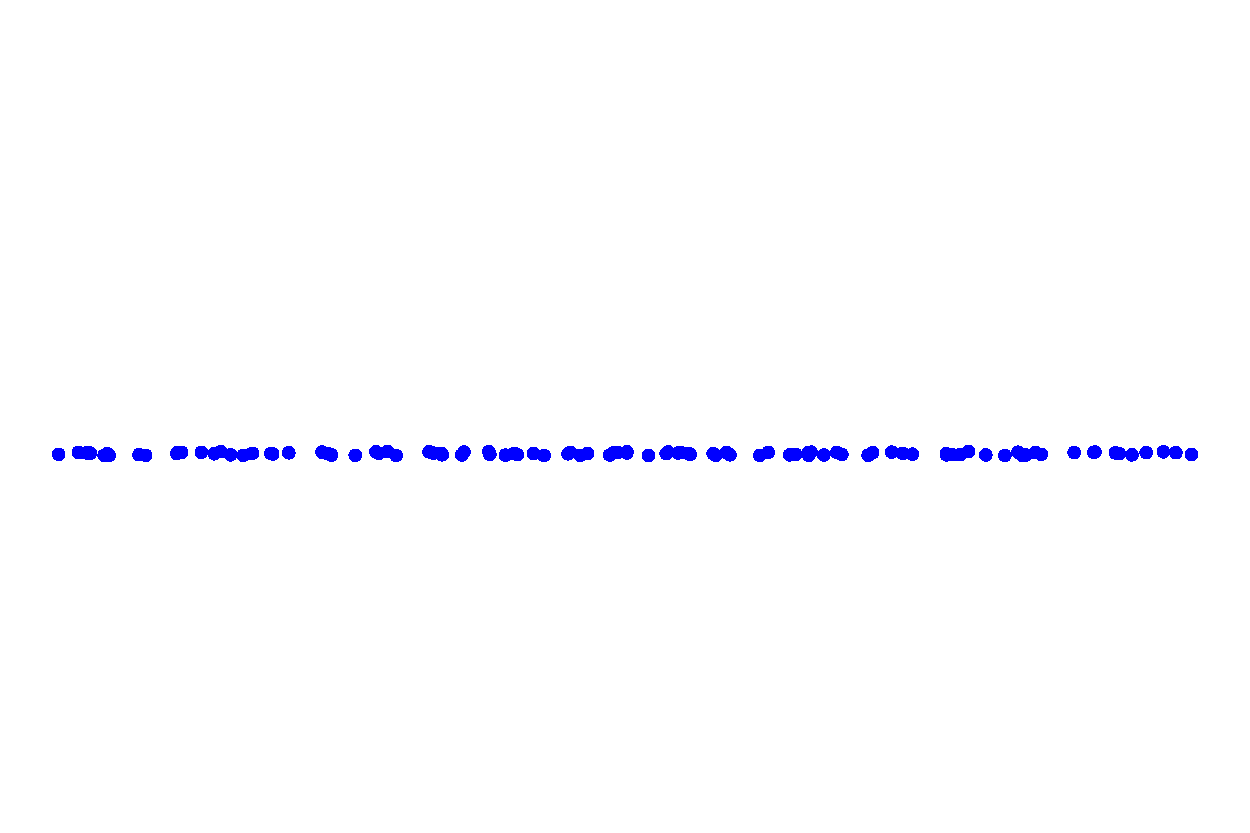
\includegraphics[trim={0 5cm 0 6cm},clip] {images/ae_code_points.pdf}};

\node[scale = .2, below of=pcacodepoints, node distance=20cm, xshift=-11cm] (pcaprojectionpoints)  {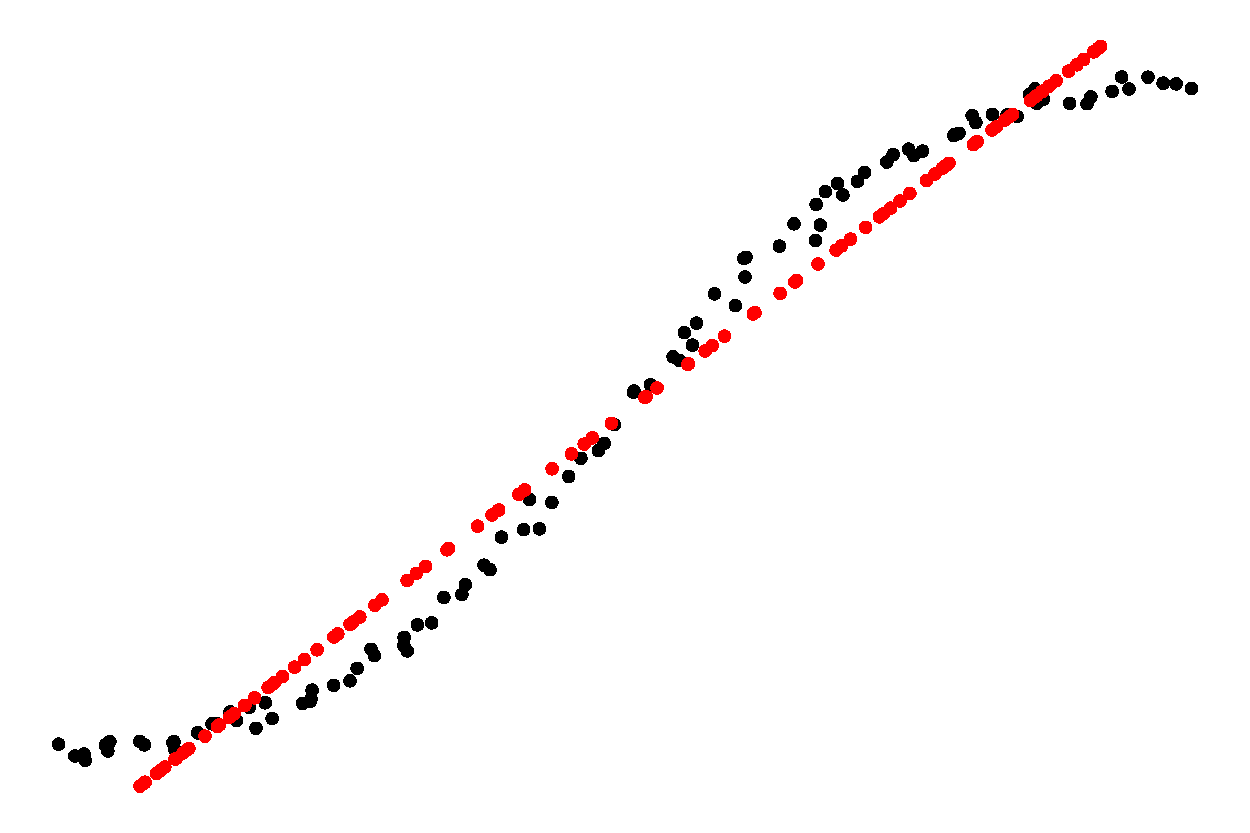
\includegraphics{images/pca_projection_points.pdf}};
\node[scale = .2, below of=aecodepoints, node distance=20cm, xshift=11cm] (aeprojectionpoints)  {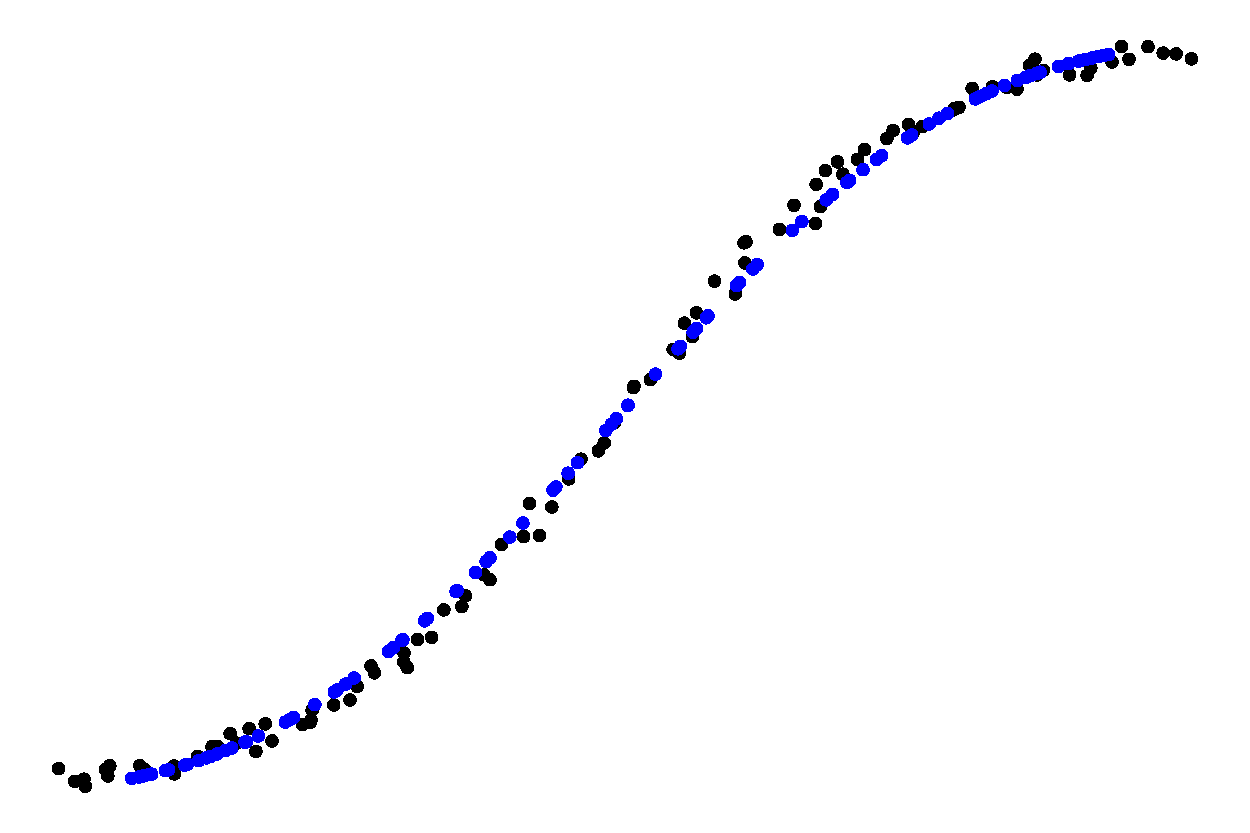
\includegraphics {images/ae_projection_points.pdf}};

%lables
\node[above of=aepoints, align=center, node distance=4cm](toutput) {\large Original Data};
\draw[-Triangle, bthickline] (aepoints) -- (pcacodepoints) node[midway, anchor=east, yshift=.2cm, align=center]{\large PCA Encoding};   
\draw[-Triangle, bthickline] (aepoints) -- (aecodepoints)node[midway, anchor=west, align=center]{\large Non-linear\\\large Encoding};
\draw[-Triangle, bthickline] (pcacodepoints) -- (pcaprojectionpoints)node[midway, anchor=east, align=center, yshift=.3cm]{\large PCA Decoding}; 
\draw[-Triangle, bthickline] (aecodepoints) -- (aeprojectionpoints)node[midway, anchor=west, align=center]{\large Non-linear\\\large Decoding};

%markings on the plots
\node[above of=pcaprojectionpoints, align=center, yshift=-0.8cm, xshift=-1cm, rotate=40](toutput) {\large Projection on a \\\large hyperplane};
\node[above of=aeprojectionpoints, align=center, yshift=-1cm, xshift=-1cm, rotate=40](toutput) {\large Projection on a \\\large manifold};

\end{tikzpicture}
\end{document}